\documentclass[11pt]{article}
\usepackage[margin=1in]{geometry}
\usepackage[T1]{fontenc}
\usepackage{lmodern}
\usepackage{amsmath,amssymb,amsthm}
\usepackage{tikz,tikz-cd,needspace}
\usepackage[section]{placeins}
\usepackage{enumitem,booktabs,tabularx,array}
\usepackage[hidelinks]{hyperref}
\usetikzlibrary{arrows.meta,patterns,calc,positioning}
\setlist{itemsep=2pt,topsep=4pt}
\theoremstyle{definition}
\newtheorem{Def}{Definition}
\newtheorem{Ex}{Example}
\newtheorem{Prop}{Proposition}
\theoremstyle{remark}
\newtheorem{Rmk}{Remark}
\DeclareMathOperator{\Spec}{Spec}
\DeclareMathOperator{\Cl}{Cl}
\DeclareMathOperator{\Pic}{Pic}
\DeclareMathOperator{\Hom}{Hom}
\DeclareMathOperator{\Tot}{Tot}
\DeclareMathOperator{\divisor}{div}
\newcommand{\A}{\mathbb A}
\newcommand{\Pj}{\mathbb P}
\newcommand{\C}{\mathbb C}
\newcommand{\Z}{\mathbb Z}
\newcommand{\R}{\mathbb R}
\newcommand{\Gm}{\mathbb G_m}
\newcommand{\OO}{\mathcal O}
\newcommand{\Cone}[1]{\operatorname{Cone}(#1)}
\renewcommand{\figurename}{Diagram}

\begin{document}
\begin{center}
  {\Large\bfseries November 2, 2026}\\[4pt]
  {\large Cox quotients, torus torsors, and line bundles}
\end{center}

These notes follow the lecture and board images, using the notation
of Chapter~6, \emph{Cox Coordinates and Quotient Constructions}.
The main points are:
\begin{itemize}
\item Affine product descriptions can glue to a nontrivial torus torsor.
\item A character of the Cox group specifies a line bundle; its weight
      is one additional column in the action matrix.
\item The irrelevant locus removes exactly the coordinate strata
      where the torus map cannot extend to a toric morphism.
\item Quotients are constructed from invariant regular functions.
      Smooth, simplicial, and nonsimplicial fans give different orbit behavior.
\end{itemize}

\section{Notation and the Cox construction}

Work over \(\C\). Let \(N\cong\Z^d\) be the lattice of
\emph{one-parameter subgroups}, \(M=\Hom(N,\Z)\) its character
lattice, and \(\Sigma\) a fan whose rays span \(N_\R\). Put
\(r=|\Sigma(1)|\), and write \(u_\rho\) for a primitive ray generator.
The two lattice maps are
\[
\begin{aligned}
\beta:\Z^r&\longrightarrow N,&e_\rho&\longmapsto u_\rho,\\
\beta^*:M&\longrightarrow\Z^r,&m&\longmapsto
       (\langle m,u_\rho\rangle)_\rho.
\end{aligned}
\]
\begin{Rmk}[The lattice convention on the board]
The map sending standard basis vectors to ray generators is a map
of \(N\)-lattices. Some board labels call these spaces \(M\).
Here we use Chapter~6's convention: cones lie in \(N_\R\), while
characters and semigroup coordinate rings use \(M\).
\end{Rmk}

Recall the divisor-class sequence and its diagonal group:
\[
0\longrightarrow M\xrightarrow{\beta^*}\Z^r
 \xrightarrow{\deg}\Cl(X_\Sigma)\longrightarrow0,
\qquad
G=\Hom(\Cl(X_\Sigma),\Gm).
\]
The Cox ring, irrelevant ideal, and Cox open set are
\[
\begin{aligned}
S&=\C[x_\rho:\rho\in\Sigma(1)],
       &\deg(x_\rho)&=[D_\rho],\\
B(\Sigma)&=\left\langle x^{\widehat\sigma}:
                  \sigma\in\Sigma_{\max}\right\rangle,
       &x^{\widehat\sigma}&=\prod_{\rho\notin\sigma(1)}x_\rho,\\
Z(\Sigma)&=V(B(\Sigma)),
       &\widehat X_\Sigma&=\A^r\setminus Z(\Sigma).
\end{aligned}
\]
The quotient morphism is
\[
\pi:\widehat X_\Sigma\longrightarrow X_\Sigma,
\qquad
X_\Sigma\cong\widehat X_\Sigma\mathbin{//}G.
\]
The symbol \(Z(\Sigma)\) denotes a zero set, whereas \(\Z\) denotes
the integers. We remove \(V(B)\); we do not replace \(S\) by \(S/B\).

\section{Local products need not give a global product}

% Board 1: the clarification about affine products and global torsors.
Suppose a surjective lattice map
\(\beta:\widehat N\twoheadrightarrow N\), with kernel \(K\),
identifies a cone \(\widehat\sigma\) with \(\sigma\) and identifies
their saturated span lattices integrally. An adapted splitting gives
\[
(\widehat N,\widehat\sigma)
 \cong(N\oplus K,\sigma\times\{0\}),\qquad
U_{\widehat\sigma}\cong U_\sigma\times T_K,
\]
where \(T_K\cong(\Gm)^{\operatorname{rank}K}\).
This follows by taking dual semigroup algebras: the kernel directions
contribute invertible Laurent variables. The splitting is a choice,
so the product is not canonical.

For a smooth Cox fan, with \(\beta:\Z^r\to N\) surjective, this yields
\[
\pi^{-1}(U_\sigma)\cong U_\sigma\times(\Gm)^{r-d}.
\]
Different chartwise splittings can have nonconstant transition
functions. Consequently, the global conclusion is a
\emph{torus torsor over} \(X_\Sigma\), not necessarily a product.

\begin{Def}[Torus torsor in the setting of the lecture]
A Zariski locally trivial \(T\)-torsor \(P\to X\) is a space with a
\(T\)-action and an open cover \(\{U_i\}\) such that
\[
P|_{U_i}\cong U_i\times T
\]
equivariantly, with \(T\) acting on itself by multiplication. On each
fiber the action is free and transitive. The torsor is globally
trivial exactly when it admits a global section.
\end{Def}

\begin{Rmk}[Hypothesis behind the torus-bundle statement]
For the smooth torus-bundle statements we assume that \(\beta\) is
surjective on lattices. This holds if the smooth fan has a
full-dimensional cone, as in the lecture examples. It implies that
\(\Cl(X)\) is free and \(G\cong(\Gm)^{r-d}\).
Smoothness alone, for arbitrary noncomplete fans, does not force the
global class group to be torsion free. Without the additional
hypothesis the smooth Cox quotient is a torsor under a diagonalizable
group, locally trivial in the appropriate \emph{\'etale} topology;
it need not be a Zariski torus torsor.
\end{Rmk}

\subsection{The first example already has nontrivial gluing}

For \(\Pj^1\), the Cox map is
\[
\pi:\A^2\setminus\{0\}\longrightarrow\Pj^1,
\qquad (x,y)\longmapsto[x:y].
\]
Its fibers are scalar orbits, each isomorphic to \(\Gm\). The map
\[
(x,y)\longmapsto\bigl([x:y],(x,y)\bigr)
\]
identifies its source with the tautological line bundle with its
zero section removed:
\[
\boxed{\A^2\setminus\{0\}
 \cong\Tot\OO_{\Pj^1}(-1)\setminus0_{\Pj^1}.}
\]
Here the fiber of \(\OO(-1)\) over a line \(\ell\subset\C^2\)
is the line \(\ell\) itself.

On \(U_0=\{x\ne0\}\), use base coordinate \(u=y/x\) and fiber
coordinate \(a=x\). On \(U_1=\{y\ne0\}\), use \(v=x/y\) and
\(b=y\). The overlap transformation is
\[
\boxed{v=u^{-1},\qquad b=ua.}
\]
The fiber transition depends on the base coordinate. The torsor is
not \(\Pj^1\times\Gm\) over \(\Pj^1\): a section would give a
nowhere-zero regular section of \(\OO(-1)\), whereas
\(H^0(\Pj^1,\OO(-1))=0\).

\begin{figure}[htbp]
\centering
\begin{tikzcd}[column sep=huge,row sep=large]
\pi^{-1}(U_0)\cong\A^1_u\times\Gm
 \arrow[d,"\pi"']
 \arrow[r,dashed,"{(u,a)\mapsto(u^{-1},ua)}"]
&\pi^{-1}(U_1)\cong\A^1_v\times\Gm\arrow[d,"\pi"]\\
U_0\cong\A^1_u\arrow[r,dashed,"u\mapsto u^{-1}"']
&U_1\cong\A^1_v
\end{tikzcd}
\caption{The dashed coordinate changes are defined on the overlaps,
where \(u,v\ne0\). Each chart is a product, but the fiber gluing
\(b=ua\) gives the nontrivial punctured tautological bundle.}
\label{fig:nov02-torsor-gluing}
\end{figure}

% Board 2: a character specifies the action on one additional coordinate.
\section{Line bundles from one additional Cox coordinate}
\label{sec:nov02-associated-line-bundles}

Continue in the smooth setting, where the Cox quotient
\(\pi:\widehat X\to X_\Sigma\) is the torsor discussed above.
For a divisor class \(\alpha\in\Pic(X_\Sigma)=\Cl(X_\Sigma)\),
evaluation defines a character
\[
\chi_\alpha:G\longrightarrow\Gm,\qquad
\chi_\alpha(g)=g(\alpha).
\]
Add one affine coordinate \(z\), and let
\[
g\cdot(x,z)=\bigl(g\cdot x,\chi_\alpha(g)z\bigr).
\]
Then
\[
\boxed{
\Tot\OO_{X_\Sigma}(D)
\cong(\widehat X\times\A^1)/G,
\qquad [D]=\alpha.
}
\]
The projection to \(X_\Sigma\) sends \([x,z]\) to \(\pi(x)\),
and \([x,0]\) defines the zero section. Thus the quotient is the
\emph{total space} of the line bundle, rather than its base.

\begin{figure}[htbp]
\centering
\begin{tikzcd}[row sep=large,column sep=large]
\widehat X\times\A^1
  \arrow[r,"{/G}"]\arrow[d,"\operatorname{pr}_1"']
  &\Tot\OO(D)\arrow[d,"p"]\\
\widehat X\arrow[r,"\pi"']&X_\Sigma
\end{tikzcd}
\caption{A character of the Cox group determines the action on the
extra coordinate. The quotient of a trivial line upstairs can be a
nontrivial line bundle downstairs.}
\label{fig:nov02-associated-bundle}
\end{figure}

\subsection{Local coordinates verify the construction}

Choose an invariant representative
\(D=\sum_\rho a_\rho D_\rho\). For a maximal cone \(\sigma\),
let \(m_\sigma\) be its Cartier datum:
\[
\langle m_\sigma,u_\rho\rangle=-a_\rho
\qquad(\rho\subseteq\sigma).
\]
On the Cox chart
\(\widehat U_\sigma=D(x^{\widehat\sigma})\), set
\[
q_\sigma=
\prod_\rho x_\rho^{a_\rho+\langle m_\sigma,u_\rho\rangle}.
\]
Its exponents on rays inside \(\sigma\) are zero; coordinates on
the other rays are invertible on this chart. Thus \(q_\sigma\)
is an invertible Laurent monomial of degree \(\alpha\), with
\(q_\sigma(gx)=\chi_\alpha(g)q_\sigma(x)\). Consequently,
\[
w_\sigma=\frac{z}{q_\sigma}
\]
is invariant, and the local quotient is
\[
\Spec\bigl(\OO(U_\sigma)[w_\sigma]\bigr)
\cong U_\sigma\times\A^1.
\]
On overlaps,
\[
w_\tau=\frac{q_\sigma}{q_\tau}w_\sigma
=\chi^{m_\sigma-m_\tau}w_\sigma.
\]
These are the fiber-coordinate transitions of \(\OO(D)\): its local
frames satisfy \(e_\sigma=\chi^{m_\sigma-m_\tau}e_\tau\).
This verifies the bundle and fixes the sign of the extra weight.

\subsection{The extra column in the weight matrix}

Suppose \(G\cong\Gm^k\), and let \(Q=(q_{i\rho})\) be the
\(k\times r\) Cox weight matrix. Its \(\rho\)-th column records
\([D_\rho]\) in the chosen basis of \(\Cl(X_\Sigma)\). Thus
\[
(t_1,\ldots,t_k)\cdot x_\rho
=\left(\prod_{i=1}^k t_i^{q_{i\rho}}\right)x_\rho.
\]
Writing \(a=(a_\rho)\), the class of \(D\) is the column \(Qa\).
The action on the new coordinate is
\[
z\longmapsto\left(\prod_{i=1}^k t_i^{(Qa)_i}\right)z,
\qquad
\boxed{Q_L=(Q\mid Qa).}
\]
This is the lecture's rule: add the same linear combination of the
old columns as the divisor's linear combination of boundary classes.
The admissible open set remains \(\widehat X\times\A^1\);
the irrelevant ideal extends from \(S\) to \(S[z]\).

\begin{Ex}[Calibrating on \(\Pj^1\)]
For \(\OO_{\Pj^1}(n)\), use
\[
\lambda\cdot(x_0,x_1,z)
=(\lambda x_0,\lambda x_1,\lambda^n z),
\qquad Q_L=(1\ \ 1\ \ n).
\]
On \(x_i\ne0\), the invariant fiber coordinate is
\(w_i=z/x_i^n\). Hence
\[
w_1=\left(\frac{x_0}{x_1}\right)^n w_0,
\]
which is the transition for \(\OO(n)\). The exponent is \(+n\)
for the simultaneous action used here. A homogeneous Cox polynomial
\(f\) of degree \([D]\) similarly gives a section
\(\pi(x)\mapsto[x,f(x)]\), since \(f\) transforms like \(z\).
\end{Ex}

% Board 3: the fan adds a vertical ray and the column of negative coefficients.
\section{Fan of the total space}
\label{sec:nov02-line-bundle-fan}

The quotient has an explicit fan in
\(N_L=N\oplus\Z\). For each base ray and for the zero section, take
\[
\widetilde u_\rho=(u_\rho,-a_\rho),\qquad
u_z=(0,1).
\]
For every \(\sigma\in\Sigma\), form
\[
\widetilde\sigma=
\Cone{\{\widetilde u_\rho:\rho\subseteq\sigma\}\cup\{u_z\}},
\]
and include all faces. These cones make the fan of \(\Tot\OO(D)\).
The projection \((v,t)\mapsto v\) induces its bundle map; the
vertical ray \(u_z\) corresponds to the zero-section divisor.

If the \(r\times d\) matrix \(A\) has rows \(u_\rho\), the
augmented ray matrix is
\[
\boxed{
A_L=
\begin{pmatrix}
 A&-a\\
 0&1
\end{pmatrix}.
}
\]
It also gives the character-lattice map
\(M\oplus\Z\to\Z^{r+1}\). The two matrix recipes are compatible:
\[
Q_LA_L=(Q\mid Qa)
\begin{pmatrix}A&-a\\0&1\end{pmatrix}=0,
\]
because \(QA=0\).

\subsection{Local products and changing the divisor representative}

On \(\sigma\), the lifted base rays lie on the graph
\(t=\langle m_\sigma,v\rangle\). Thus
\[
\widetilde\sigma
=\{(v,t):v\in\sigma,\ t\geq\langle m_\sigma,v\rangle\}.
\]
The integral shear
\((v,t)\mapsto(v,t-\langle m_\sigma,v\rangle)\) identifies this
cone with \(\sigma\times\R_{\geq0}\), proving the local product
\(p^{-1}(U_\sigma)\cong U_\sigma\times\A^1\).
The character \((-m_\sigma,1)\) supplies its fiber coordinate.

If \(D'=D+\divisor(\chi^m)\), then
\(a'_\rho=a_\rho+\langle m,u_\rho\rangle\). The global lattice
automorphism
\[
(v,t)\longmapsto(v,t-\langle m,v\rangle)
\]
sends the fan for \(D\) to that for \(D'\), fixes \((0,1)\), and
preserves projection to the base. Also \(Qa'=Qa\), so the extra Cox
weight depends only on the line-bundle class.

\begin{Ex}[Two representatives of \(\OO_{\Pj^1}(n)\)]
Let the base rays be \(+1,-1\), with divisors \(D_0,D_\infty\).
For \(D=nD_\infty\), the lifted rays are
\[
(1,0),\qquad(-1,-n),\qquad(0,1).
\]
The maximal cones pair the vertical ray with each of the other two.
For \(D'=nD_0\), the rays instead are
\[
(1,-n),\qquad(-1,0),\qquad(0,1).
\]
The shear \((v,t)\mapsto(v,t-nv)\) identifies these fans, reflecting
\(nD_0\sim nD_\infty\). A change of lattice coordinates must act on
the whole fan, rather than on an individual ray.
\end{Ex}

% Lecture image 2: the fan of the total space of O_{P^1}(n), shown for n=2.
\begin{figure}[htbp]
\centering
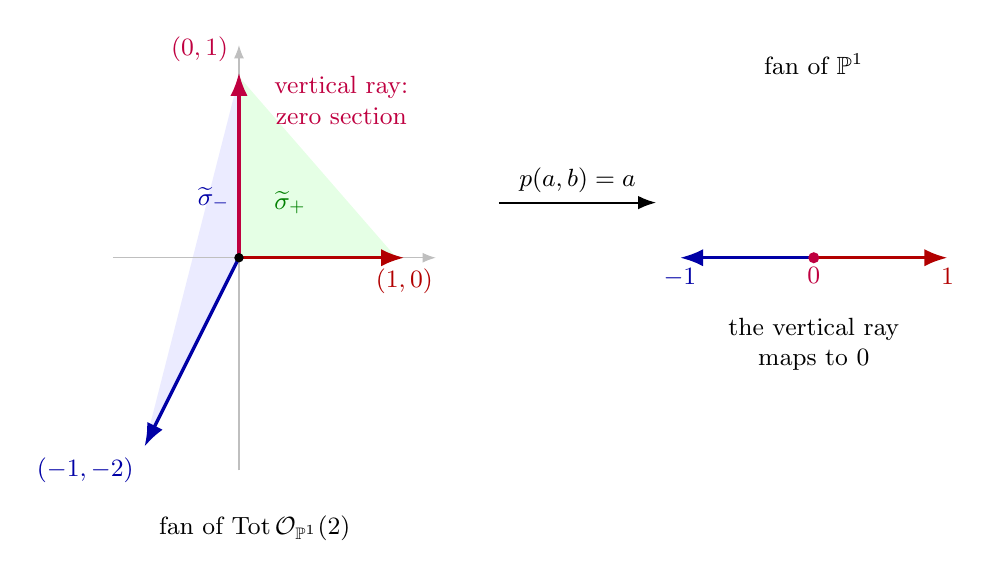
\begin{tikzpicture}[font=\small,>=Latex,line join=round]
  \begin{scope}[xshift=-3.2cm]
    \fill[green!10] (0,0)--(2,0)--(0,2.3)--cycle;
    \fill[blue!8] (0,0)--(0,2.3)--(-1.2,-2.4)--cycle;
    \draw[->,gray!50] (-1.6,0)--(2.5,0);
    \draw[->,gray!50] (0,-2.7)--(0,2.7);
    \draw[->,very thick,red!70!black] (0,0)--(2.1,0)
      node[below] {$(1,0)$};
    \draw[->,very thick,blue!65!black] (0,0)--(-1.2,-2.4)
      node[below left] {$(-1,-2)$};
    \draw[->,very thick,purple] (0,0)--(0,2.35)
      node[above left] {$(0,1)$};
    \fill (0,0) circle (1.7pt);
    \node[green!50!black] at (0.65,0.7) {$\widetilde\sigma_+$};
    \node[blue!65!black] at (-0.32,0.75) {$\widetilde\sigma_-$};
    \node[purple,align=center] at (1.3,2)
      {vertical ray:\\zero section};
    \node[below] at (0.2,-3.15)
      {fan of $\operatorname{Tot}\mathcal O_{\mathbb P^1}(2)$};
  \end{scope}
  \draw[->,thick] (0.1,0.7)--(2.1,0.7)
    node[midway,above] {$p(a,b)=a$};
  \begin{scope}[xshift=4.1cm]
    \draw[->,very thick,blue!65!black] (0,0)--(-1.7,0)
      node[below] {$-1$};
    \draw[->,very thick,red!70!black] (0,0)--(1.7,0)
      node[below] {$1$};
    \fill[purple] (0,0) circle (2pt);
    \node[below,purple] at (0,0) {$0$};
    \node[above] at (0,2.2) {fan of $\mathbb P^1$};
    \node[align=center] at (0,-1.1)
      {the vertical ray\\maps to $0$};
  \end{scope}
\end{tikzpicture}
\caption{The line-bundle fan in the convention of Chapter 6. For
$D=2D_{-1}$, the lifted rays are $(1,0)$ and $(-1,-2)$, together with
the vertical ray $(0,1)$. Each maximal cone contains that vertical
ray; projection onto the first coordinate is the bundle map.}
\label{fig:nov02-linebundle-fan}
\end{figure}

\section{Why remove the irrelevant locus? The fan explanation}

% Boards 4--5: compatible coordinate cones and the distinguished-point argument.
The fan of \(\A^r\) consists of all faces of the positive orthant.
For \(I\subseteq\Sigma(1)\), let
\[
\tau_I=\Cone{e_\rho:\rho\in I}.
\]
A lattice map defines a toric morphism exactly when every source
cone maps into a target cone. Thus we keep precisely the faces
\(\tau_I\) for which
\[
\beta(\tau_I)\subseteq\sigma
\quad\text{for some }\sigma\in\Sigma.
\]
Since the \(u_\rho\) are rays of the same fan, this is equivalent
to \(I\subseteq\sigma(1)\). The resulting source subfan is
\[
\widehat\Sigma
=\{\tau_I:I\subseteq\sigma(1)\text{ for some }\sigma\in\Sigma\}.
\]
Its toric variety is exactly \(\widehat X_\Sigma\). It is the largest
torus-invariant open subset of this \(\A^r\) on which the given
torus map extends regularly to \(X_\Sigma\).

The orbit closure of \(\tau_I\) in \(\A^r\) is
\[
V(\tau_I)=V(x_\rho:\rho\in I).
\]
If \(I\) is forbidden, every larger set is forbidden as well, and
its coordinate subspace is already contained in this one. Hence
\[
Z(\Sigma)
=\bigcup_{\substack{P\text{ minimal}\\
             P\not\subseteq\sigma(1)\text{ for all }\sigma}}
              V(x_\rho:\rho\in P).
\]
These minimal forbidden ray sets are the \emph{primitive collections}
in Chapter~6. This explains the minimal-set description of the
irrelevant locus through the orbit--cone correspondence.

% Lecture images 4--5: cone compatibility explains the deleted locus.
\begin{figure}[htbp]
\centering
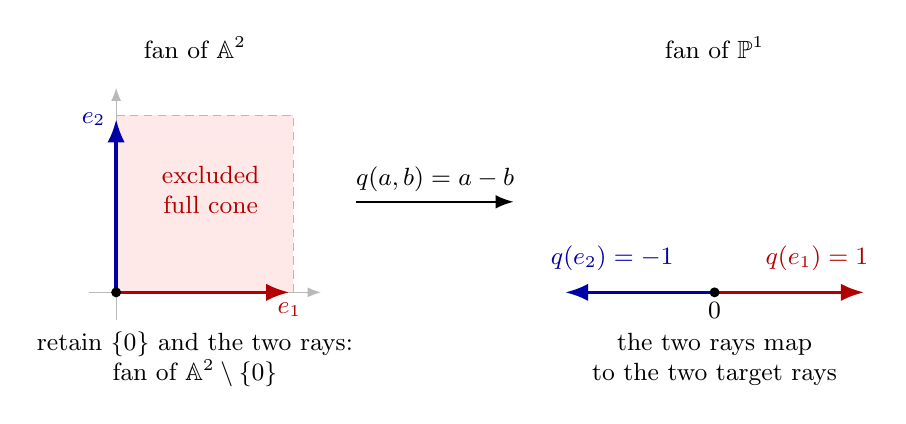
\begin{tikzpicture}[font=\small,>=Latex,line join=round]
  \begin{scope}[xshift=-3.6cm]
    \fill[red!9] (0,0)--(2.25,0)--(2.25,2.25)--(0,2.25)--cycle;
    \draw[gray!55,densely dashed] (2.25,0)--(2.25,2.25)--(0,2.25);
    \draw[->,gray!55] (-0.35,0)--(2.6,0);
    \draw[->,gray!55] (0,-0.35)--(0,2.6);
    \draw[->,very thick,red!70!black] (0,0)--(2.2,0)
      node[below] {$e_1$};
    \draw[->,very thick,blue!65!black] (0,0)--(0,2.2)
      node[left] {$e_2$};
    \fill (0,0) circle (1.8pt);
    \node[align=center,red!70!black] at (1.2,1.3)
      {excluded\\full cone};
    \node[above] at (1,2.85) {fan of $\mathbb A^2$};
    \node[align=center] at (1,-0.85)
      {retain $\{0\}$ and the two rays:\\fan of $\mathbb A^2\setminus\{0\}$};
  \end{scope}
  \draw[->,thick] (-0.55,1.15)--(1.45,1.15)
    node[midway,above] {$q(a,b)=a-b$};
  \begin{scope}[xshift=4cm]
    \draw[->,very thick,blue!65!black] (0,0)--(-1.9,0);
    \draw[->,very thick,red!70!black] (0,0)--(1.9,0);
    \fill (0,0) circle (1.8pt);
    \node[above,blue!65!black] at (-1.3,0.15) {$q(e_2)=-1$};
    \node[above,red!70!black] at (1.3,0.15) {$q(e_1)=1$};
    \node[below] at (0,0) {$0$};
    \node[above] at (0,2.85) {fan of $\mathbb P^1$};
    \node[align=center] at (0,-0.85)
      {the two rays map\\to the two target rays};
  \end{scope}
\end{tikzpicture}
\caption{The cocharacter map for the Cox quotient of $\mathbb P^1$.
The full positive quadrant maps onto the whole real line, which is
not contained in either cone of the target fan. Removing its orbit,
the origin of $\mathbb A^2$, leaves a fan-compatible map.}
\label{fig:nov02-cox-fan}
\end{figure}

\begin{Ex}[Why the origin of \(\A^2\) must be removed]
For \(\Pj^1\), the lattice map is
\(\beta(a,b)=a-b\). The full positive quadrant maps to all of
\(\R\), which is not contained in either cone of the fan of
\(\Pj^1\). Algebraically, the map \([x:y]\) has no regular extension
at the origin: both curves
\[
t\longmapsto(t^2,t),\qquad
t\longmapsto(t,t^2)
\]
approach \((0,0)\), but their projective images approach \([0:1]\)
and \([1:0]\), respectively. A morphism cannot give one point two
different images.
The torus map therefore defines a \emph{rational map} with an
indeterminacy at the origin. Arbitrary set-theoretic assignments at
that point would not repair regularity. This is the precise meaning
of the lecture's statement that the map is not defined there.
\end{Ex}

\section{Quotients through invariant regular functions}

% Boards 6--8: functions constant on orbits and intersecting orbit closures.
Suppose \(G\) acts on a variety \(Y\). A function on an orbit space
must pull back to a function \(F\) satisfying
\[
F(g\cdot y)=F(y)\qquad(g\in G).
\]
Such a function is \emph{invariant}. It is also equivariant if its
target \(\A^1\) is given the trivial action. Set-theoretically,
invariance makes \(f([y])=F(y)\) well defined; an algebraic quotient
must also have the correct regular functions and topology.

If \(Y=\Spec A\) is affine and \(G\) is reductive over \(\C\), the
invariant algebra is finitely generated, and the affine quotient is
\[
\boxed{Y\mathbin{//}G=\Spec(A^G).}
\]
The lecture's groups \((\Gm)^k\) and finite diagonalizable factors
are included. Here \(A\) is the ring of \emph{regular} functions,
not merely the rational function field.

Why can this quotient identify distinct orbits? If \(F\) is
constant with value \(c\) on an orbit, the closed set \(F^{-1}(c)\)
contains its closure. Thus two orbit closures meeting at one point
have equal values under every invariant regular function. For an
affine reductive action, each quotient fiber contains a unique closed
orbit; the other orbits in that fiber have closures containing it.

\begin{figure}[htbp]
\centering
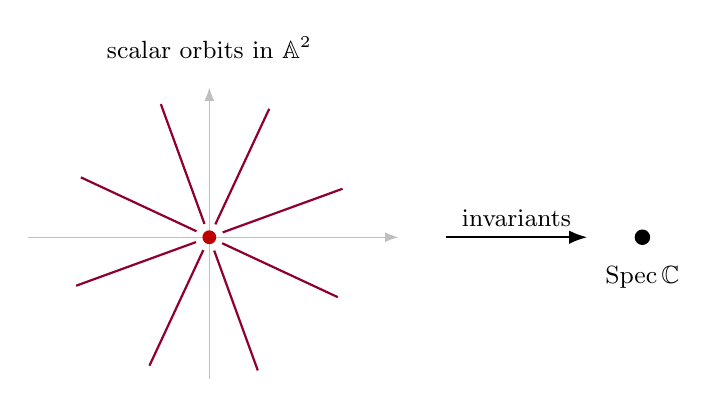
\begin{tikzpicture}[>=Latex,font=\small]
  \draw[gray!50,->] (-2.3,0)--(2.4,0);
  \draw[gray!50,->] (0,-1.8)--(0,1.9);
  \foreach \ang in {20,65,110,155} {
    \draw[purple!75!black,thick] (\ang:0.18)--(\ang:1.8);
    \draw[purple!75!black,thick] (\ang+180:0.18)--(\ang+180:1.8);
  }
  \fill[red!75!black] (0,0) circle (2.5pt);
  \node[above] at (0,2.15) {scalar orbits in \(\A^2\)};
  \draw[->,thick] (3,0)--(4.8,0)
     node[midway,above] {invariants};
  \fill (5.5,0) circle (2.8pt);
  \node[below] at (5.5,-0.25) {\(\Spec\C\)};
\end{tikzpicture}
\caption{Real slices of several complex scalar orbits. Each punctured
line has the origin in its closure; the origin is a separate orbit.
All invariant polynomial functions take the same value on all of them.}
\label{fig:nov02-orbit-closures}
\end{figure}

\subsection{Good and geometric quotients}

For the reductive actions in this lecture, a \emph{good quotient}
\(\pi:Y\to Q\) is an invariant affine surjection with
\[
\OO_Q=(\pi_*\OO_Y)^G,
\]
which sends invariant closed subsets to closed subsets and sends
disjoint invariant closed subsets to disjoint subsets. The sheaf
condition means that regular functions on every open subset of
\(Q\) are exactly the invariant regular functions on its inverse
image. In our Cox construction this is checked by taking invariants
on affine charts and gluing.

For a good Cox quotient, being \emph{geometric} additionally means
that every fiber is a single \(G\)-orbit. The Cox theorem says
\[
\boxed{\widehat X_\Sigma\mathbin{//}G
\text{ is geometric}\quad\Longleftrightarrow\quad
\Sigma\text{ is simplicial}.}
\]
This is why the double slash is useful before one has established
the orbit statement. General definitions of geometric quotients
also specify the quotient topology and invariant-function sheaf;
geometric quotients in other settings need not be affine morphisms.

\subsection{Recovering \texorpdfstring{\(\Pj^1\)}{P1} by deleting, localizing, and gluing}

Let \(\Gm\) act on \(\A^2\) by
\(t\cdot(x,y)=(tx,ty)\). A nonconstant monomial \(x^ay^b\)
has positive weight \(a+b\), so
\[
\C[x,y]^{\Gm}=\C,\qquad
\A^2\mathbin{//}\Gm=\Spec\C.
\]
The nonzero vectors have many different orbits, but every orbit
closure contains the origin. This affine quotient is a point,
rather than \(\Pj^1\).

Remove the origin. The open set \(\A^2\setminus\{0\}\) is not
affine, so take a \(G\)-stable affine cover and compute locally:
\[
\begin{array}{c|c|c}
\text{open upstairs}&\text{coordinate ring}&\text{invariant ring}\\ \hline
D(x)&\C[x,x^{-1},y]&\C[y/x]=\C[u]\\
D(y)&\C[x,y,y^{-1}]&\C[x/y]=\C[v]\\
D(xy)&\C[x^{\pm1},y^{\pm1}]&\C[u,u^{-1}]
\end{array}
\]
The transition \(v=u^{-1}\) glues the two quotient affine lines to
\(\Pj^1\). This is exactly the degree-zero localization construction:
the grading records the action, and degree zero records invariance.
The recording occasionally says \(\Pj^2\) here; two homogeneous
coordinates give \(\Pj^1\).

\begin{Rmk}[Global functions alone still do not recover the quotient]
Even after deleting the origin,
\[
\Gamma(\A^2\setminus\{0\},\OO)
=\C[x,x^{-1},y]\cap\C[x,y,y^{-1}]=\C[x,y]
\]
inside \(\C(x,y)\). Its invariant subring is still \(\C\).
Thus taking \(\Spec\) of the global invariant ring would again
lose \(\Pj^1\). The successful construction uses local invariant
rings and their gluing. The same computation proves the punctured
plane is nonaffine: its canonical map to the spectrum of its global
functions is the inclusion into \(\A^2\), which misses the origin.
\end{Rmk}

For a general Cox chart, the corresponding identity is
\[
\left(S_{x^{\widehat\sigma}}\right)^G
=\left(S_{x^{\widehat\sigma}}\right)_0
\cong\C[\sigma^\vee\cap M].
\]
This recovers Chapter~6's affine toric charts from the quotient.

\subsection{The construction does not imply projectivity}

The Cox quotient exists for fans that are not normal fans of
polytopes. It therefore does not, by itself, prove projectivity or
even quasiprojectivity. A toric variety is projective precisely when
its fan is complete and admits an integral strictly convex support
function. Every complete toric surface is projective; in dimension
three, complete nonprojective examples occur. This is the distinction
from Chapter~5 that arose in the lecture's question.

% Lecture transcription and final singular-fan board photographs.
\section{What changes for singular fans}
\label{sec:nov02-singular}

The Cox construction uses the class-group sequence, not just Cartier
divisors. Thus it continues to work when \(X_\Sigma\) is singular:
\[
0\longrightarrow M\longrightarrow\Z^{\Sigma(1)}
\longrightarrow\Cl(X_\Sigma)\longrightarrow0,
\qquad
G=\Hom(\Cl(X_\Sigma),\Gm).
\]
As before, assume the rays span \(N_\R\), so there is no torus factor.
For a smooth variety \(\Pic(X)=\Cl(X)\); for a singular variety,
Weil-divisor classes need not represent line bundles.

If \(\Cl(X)\cong\Z^k\oplus A_{\mathrm{tors}}\), then
\[
G\cong\Gm^k\times\Hom(A_{\mathrm{tors}},\Gm).
\]
Over \(\C\), the second factor is a finite diagonalizable group.
Consequently, orbits \emph{can} be disconnected. This does not say
that every orbit is disconnected, nor that finite stabilizers require
torsion in the global class group.

For a Cox point \(z=(z_\rho)\), let
\[
L(z)=\left\langle[D_\rho]:z_\rho\ne0\right\rangle
\subseteq\Cl(X).
\]
The nonzero coordinates constrain which rescalings can fix \(z\),
giving the formula
\[
\boxed{G_z\cong\Hom\bigl(\Cl(X)/L(z),\Gm\bigr).}
\]
At the distinguished point \(z_\sigma\), whose coordinates are zero
on \(\sigma(1)\) and one elsewhere, this becomes
\[
G_{z_\sigma}\cong\Hom\bigl(\Cl(U_\sigma),\Gm\bigr).
\]
The \emph{local} class group therefore controls the stabilizer over
the orbit corresponding to \(\sigma\).

\subsection{A finite stabilizer with a connected Cox group}

Label the displayed rays, in matrix order, by
\[
u_1=(1,0),\qquad u_2=(0,1),\qquad u_3=(-2,1),
\]
and take maximal cones
\(\sigma_1=\Cone{u_1,u_2}\), \(\sigma_2=\Cone{u_2,u_3}\).
The first cone is smooth, whereas
\(\det(u_2,u_3)=2\), so the second is simplicial but singular.

\begin{figure}[htbp]
\centering
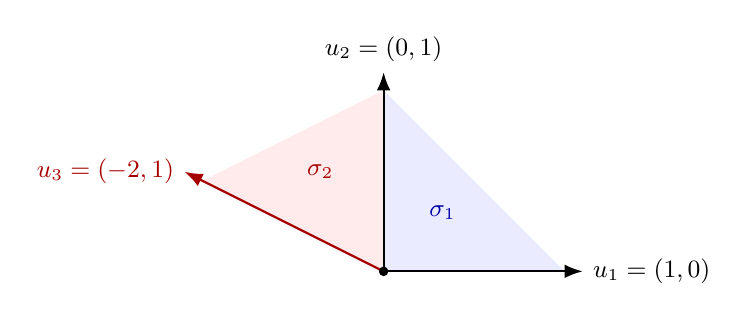
\begin{tikzpicture}[>=Latex,font=\small,scale=1.15]
  \fill[blue!8] (0,0)--(2,0)--(0,2)--cycle;
  \fill[red!8] (0,0)--(0,2)--(-2,1)--cycle;
  \draw[->,thick] (0,0)--(2.2,0)
    node[right] {$u_1=(1,0)$};
  \draw[->,thick] (0,0)--(0,2.2)
    node[above] {$u_2=(0,1)$};
  \draw[->,thick,red!65!black] (0,0)--(-2.2,1.1)
    node[left] {$u_3=(-2,1)$};
  \fill (0,0) circle (1.5pt);
  \node[blue!65!black] at (0.65,0.65) {$\sigma_1$};
  \node[red!65!black] at (-0.7,1.1) {$\sigma_2$};
\end{tikzpicture}
\caption{The two-cone fan from the lecture. Its singular cone has
index two, although the class group of the whole variety is free.}
\label{fig:nov02-finite-stabilizer-fan}
\end{figure}

The character-divisor matrix and degree map are
\[
0\longrightarrow\Z^2
\xrightarrow{\left[\begin{smallmatrix}1&0\\0&1\\-2&1\end{smallmatrix}\right]}
\Z^3\xrightarrow{(2,-1,1)}\Z\longrightarrow0.
\]
Indeed, \(\ker(2,-1,1)=\{(a,b,-2a+b):a,b\in\Z\}\).
Writing \(H=[D_3]\), the relations are
\[
[D_1]=2H,\qquad[D_2]=-H,\qquad\Cl(X)=\Z H.
\]
Thus the quotient data are
\[
\begin{gathered}
G=\Gm,\qquad
\lambda\cdot(x_1,x_2,x_3)
=(\lambda^2x_1,\lambda^{-1}x_2,\lambda x_3),\\
B=(x_1,x_3),\qquad
\widehat X=\A^3\setminus V(x_1,x_3).
\end{gathered}
\]
The point \(z_{\sigma_2}=(1,0,0)\) is fixed exactly when
\(\lambda^2=1\), so its stabilizer is \(\mu_2\).
Equivalently,
\[
\Cl(U_{\sigma_2})=\Cl(X)/\langle[D_1]\rangle
\cong\Z/2\Z.
\]
One can see the singularity directly on the chart \(x_1\ne0\):
\[
\C[x_1^{\pm1},x_2,x_3]^G
=\C[x_1x_2^2,x_2x_3,x_3^2/x_1]
\cong\C[A,B,C]/(AC-B^2).
\]

\begin{Rmk}[Correction to the displayed class group]
For the rays in Diagram~\ref{fig:nov02-finite-stabilizer-fan}, the
global class group is \(\Z\), rather than the board's
\(\Z\oplus\Z/2\Z\). The first two rows of the character matrix
already have determinant one, ruling out torsion in its cokernel.
The \(\Z/2\Z\) is the \emph{local} class group at the singular
chart, and it correctly predicts the stated \(\mu_2\) stabilizer.
This records the discrepancy for comparison with the forthcoming
instructor handout without changing the pictured fan.
\end{Rmk}

\Needspace{9cm}
\subsection{A nonsimplicial cone: several orbits in one fiber}

The final example has ray generators
\[
u_1=(0,0,1),\quad u_2=(1,0,1),\quad
u_3=(1,1,1),\quad u_4=(0,1,1).
\]
They span a three-dimensional cone over a square. Four rays in
dimension three make it nonsimplicial.

% Final lecture image: a three-dimensional non-simplicial cone.
\begin{figure}[htbp]
\centering
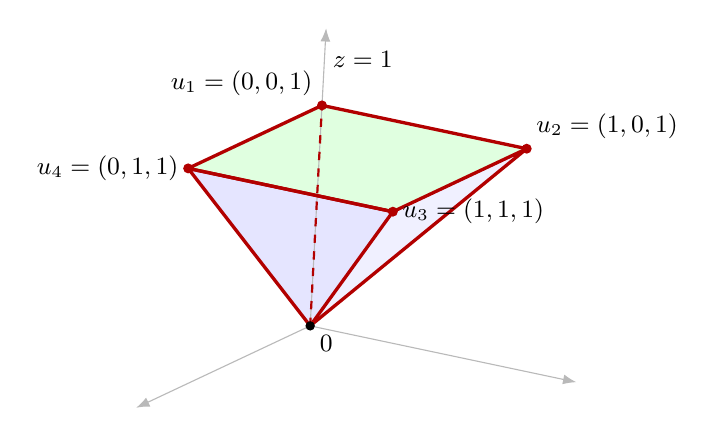
\begin{tikzpicture}[
  font=\small,line join=round,>=Latex,
  x={(2.6cm,-0.55cm)},y={(-1.7cm,-0.8cm)},z={(0.15cm,2.8cm)}]
  \coordinate (O) at (0,0,0);
  \coordinate (A) at (0,0,1);
  \coordinate (B) at (1,0,1);
  \coordinate (C) at (1,1,1);
  \coordinate (D) at (0,1,1);
  \fill[blue!6] (O)--(B)--(C)--cycle;
  \fill[blue!10] (O)--(C)--(D)--cycle;
  \fill[green!12] (A)--(B)--(C)--(D)--cycle;
  \draw[->,gray!55] (O)--(1.3,0,0);
  \draw[->,gray!55] (O)--(0,1.3,0);
  \draw[->,gray!55] (O)--(0,0,1.35);
  \draw[red!70!black,very thick] (O)--(B)--(C)--(D)--(O);
  \draw[red!70!black,very thick] (O)--(C);
  \draw[red!70!black,thick,dashed] (O)--(A);
  \draw[red!70!black,very thick] (A)--(B);
  \draw[red!70!black,very thick] (A)--(D)--(C);
  \foreach \p in {A,B,C,D}\fill[red!70!black] (\p) circle (1.8pt);
  \fill (O) circle (1.7pt);
  \node[below right] at (O) {$0$};
  \node[above left] at (A) {$u_1=(0,0,1)$};
  \node[above right] at (B) {$u_2=(1,0,1)$};
  \node[right] at (C) {$u_3=(1,1,1)$};
  \node[left] at (D) {$u_4=(0,1,1)$};
  \node at (0.5,0.5,1.45) {$z=1$};
\end{tikzpicture}
\caption{The cone over the unit square in the plane $z=1$.
It has four extremal rays in a three-dimensional lattice, so it is
not simplicial. The relation $u_1-u_2+u_3-u_4=0$ gives the Cox weights
$(1,-1,1,-1)$. The dashed ray is hidden behind the visible faces.}
\label{fig:nov02-square-cone}
\end{figure}

The relation \(u_1-u_2+u_3-u_4=0\) gives
\(\Cl(U_\sigma)\cong\Z\), with degrees \((1,-1,1,-1)\). Hence
\[
\lambda\cdot(x_1,x_2,x_3,x_4)
=(\lambda x_1,\lambda^{-1}x_2,
  \lambda x_3,\lambda^{-1}x_4).
\]
There is one maximal cone containing every ray, so its complementary
monomial is \(1\): \(B(\Sigma)=(1)\) and nothing is deleted.

In the following display, \(B\) denotes an invariant coordinate,
whereas \(B(\Sigma)\) denotes the irrelevant ideal.
The invariant ring is generated by four \emph{monomials}
\[
A=x_1x_2,\qquad B=x_1x_4,\qquad
C=x_3x_2,\qquad D=x_3x_4,
\]
with the single \emph{binomial relation} \(AD-BC=0\). Therefore
\[
\boxed{\A^4\mathbin{//}\Gm
\cong\Spec\C[A,B,C,D]/(AD-BC).}
\]
Every invariant monomial pairs equally many positive-weight and
negative-weight variables, explaining these four generators.

The fiber over the vertex is
\[
\pi^{-1}(0)=V(x_1,x_3)\cup V(x_2,x_4).
\]
These are two coordinate planes \emph{meeting at the origin}, not
two disjoint orbits. In the punctured plane \(x_2=x_4=0\), the ratio
\([x_1:x_3]\in\Pj^1\) labels distinct scaling orbits. The other
punctured plane gives another \(\Pj^1\)-family, and the origin is a
separate fixed-point orbit. Thus the vertex fiber contains infinitely
many orbits. All their closures contain the origin, so invariant
regular functions cannot distinguish them.

\begin{center}
\small
\begin{tabularx}{\linewidth}{@{}lXX@{}}
\toprule
Fan condition & Cox stabilizers & Quotient behavior\\
\midrule
Smooth & Trivial; free \(G\)-action & Geometric: one orbit per fiber\\
Simplicial & Finite, possibly nontrivial & Still geometric\\
Nonsimplicial & Positive-dimensional at the relevant distinguished points
& Good quotient; a fiber can contain several orbits\\
\bottomrule
\end{tabularx}
\end{center}
The last example distinguishes a quotient defined by invariant
functions from a literal orbit space: the former may identify
different orbits whose closures meet.

\section*{Further examples to discuss}
\begin{enumerate}
\item Starting from the Cox weight matrix for \(\Pj^1\times\Pj^1\),
      add the fiber column for \(\OO(a,b)\) and check the chart transitions.
\item Repeat the singular surface calculation with the third ray
      \((-m,1)\), \(m\geq2\). Locate the \(\mu_m\) stabilizer and
      distinguish its local class group from the global one.
\item Compare the total-space fans of linearly equivalent divisors
      using the integral shear, and identify the zero section in each fan.
\end{enumerate}

\section*{Connections and references}
Chapter~6, Sections~6.3--6.4, supplies the irrelevant ideal and
degree-zero localization construction. Section~6.6 supplies the
stabilizer formula and the nonsimplicial quadric example. Its challenge
exercise develops the additional-coordinate construction of line
bundles used in this lecture.

For the general quotient language, see the Stacks Project entries
\href{https://stacks.math.columbia.edu/tag/04AB}{Good quotients}
and \href{https://stacks.math.columbia.edu/tag/04AD}{Geometric quotients}.
The Cox quotient theorem is Cox--Little--Schenck, \emph{Toric
Varieties}, Theorem~5.1.11; see also David Cox's
\href{https://dacox.people.amherst.edu/lectures/coxcimpa.pdf}{lectures on toric varieties}.

\end{document}
